\documentclass[12pt, twoside]{article}
\usepackage[letterpaper, margin=1in, headsep=0.5in]{geometry}
\usepackage[english]{babel}
\usepackage[utf8]{inputenc}
\usepackage{amsmath}
\usepackage{amsfonts}
\usepackage{amssymb}
\usepackage{tikz}
\usepackage{yhmath}
%\usetikzlibrary{quotes, angles}

\usepackage{graphicx}
\usepackage{enumitem}
\usepackage{multicol}

\usepackage{fancyhdr}
\pagestyle{fancy}
\fancyhf{}
\renewcommand{\headrulewidth}{0pt} % disable the underline of the header

\fancyhead[RE]{\thepage}
\fancyhead[RO]{\thepage \\ Name: \hspace{3cm}}
\fancyhead[L]{BECA / Dr. Huson / 10th Grade Geometry\\* 11 June 2019}

\begin{document}
\subsubsection*{13.8 Do Now: Cross sections, distance applications}
Use only a compass and straightedge for these constructions. [show the compass marks]
 \begin{enumerate}

   \item Construct a square, inscribed in circle $O$.
     \vspace{1cm}
     \begin{center}
     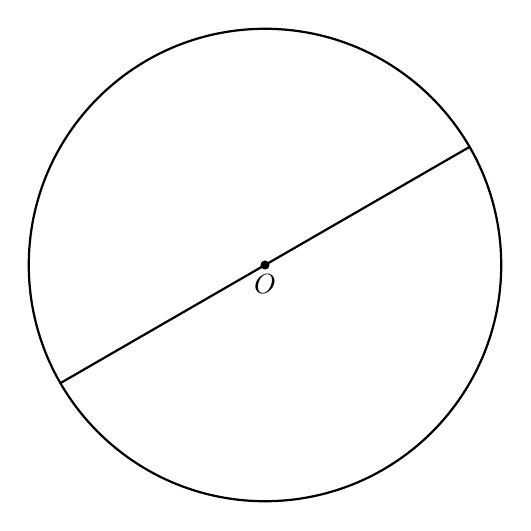
\begin{tikzpicture}
     \draw [thick] (0,0) circle [radius=3cm];
     \draw [thick] (30:3)--(210:3);
     \draw [fill] (0,0) circle [radius=0.05] node[below]{$O$};
     \end{tikzpicture}
     \end{center}
        \vspace{1cm}

   \item Construct a line through the point $P$ that is parallel to the given line $l$.
     \vspace{3cm}
     \begin{center}
     \begin{tikzpicture}
       \draw [<->, thick] (0,0)--(12,0)node[below]{$l$};
       \draw [fill] (5,-3) circle [radius=0.05] node[above left]{$P$};
     \end{tikzpicture}
   \end{center} \vspace{3cm}

\newpage

  \item Find the length of the line segment $\overline{AB}$, with $A(2,3)$ and $B(6,-1)$. Simplify the radical. \vspace{5cm}

  \item Are the given right triangles congruent? $\triangle ABC$ with $m\angle C=90^\circ$, $AC=6$, and $BC=8$. And $\triangle DEF$ with $m\angle E=90^\circ$, $DF=10$, and $EF=8$. \\[0.5cm]
  Justify your answer. \vspace{0.5cm}
    \begin{center}
      \begin{tikzpicture}[scale=0.4]
        \draw [thick] (-8.5,0)node[below]{$A$}
        --(123:8.5)node[above left]{$C$}
        --(8.5,0)node[right]{$B$}--cycle;
        %\draw (0,0) circle [radius=5] node[below]{$O$};
        \draw (123:8.5) ++(-28:0.8)-- ++(-118:0.8)-- +(152:0.8);
        \node at (70:5){8};
        \node at (150:8.5){6};
        \draw [thick] (-12,0)node[below]{$E$}
        --(-20,0)node[left]{$D$}
        --(-12,15)node[right]{$F$}--cycle;
        \draw (-12,0) ++(-180:0.8)-- ++(90:0.8)-- +(0:0.8);
        \node at (-12,7)[right]{8};
        \node at (-16.5,7)[left]{10};
      \end{tikzpicture}
   \end{center}\vspace{5cm}

\newpage
   \item Prove that $\triangle ABC$ is an isosceles triangle but not equilateral, given $A(-5,1)$, $B(5,3)$, and $C(1,-5)$, as shown below.
     \begin{multicols}{2}
       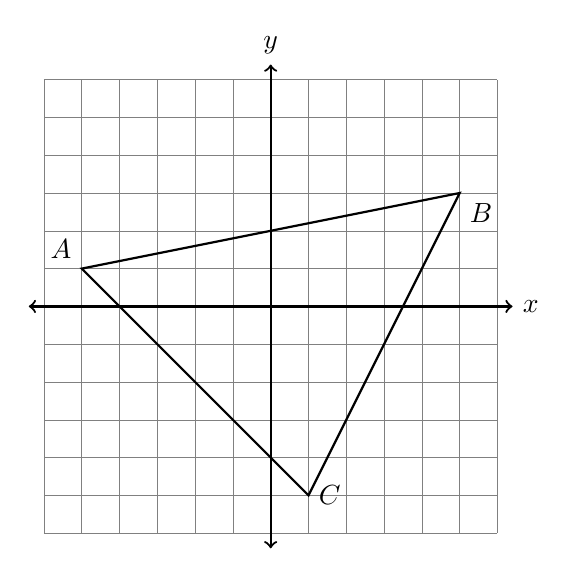
\begin{tikzpicture}[scale=.48]
         \draw [help lines] (-6,-6) grid (6,6);
         \draw [thick, <->] (-6.4,0) -- (6.4,0) node [right] {$x$};
         \draw [thick, <->] (0,-6.4)--(0,6.4) node [above] {$y$};
           \draw [thick]
           (-5,1) node[above left] {$A$}--
           (5,3) node[below right] {$B$}--
           (1,-5) node[right] {$C$}--
           cycle;
       \end{tikzpicture}
       Checklist. Confirm that you...
       \begin{itemize}
         \item Calculate lengths $AB$, $AC$ and $BC$\\
         (you do not have to simplify the radical)
         \item State which sides are congruent and which are not
         \item Write a concluding statement, that therefore $\triangle ABC$ is an isosceles triangle but not equilateral.
       \end{itemize}
     \end{multicols}

 \newpage
   \item Which three-dimensional figure will result when a rectangle 6 inches long and 5 inches wide is continuously rotated about the shorter side?
     \begin{enumerate}
       \item a rectangular prism with a length of 6 inches, width of 6 inches, and height of 5 inches
       \item a rectangular prism with a length of 6 inches, width of 5 inches, and height of 5 inches
       \item a cylinder with a radius of 5 inches and a height of 6 inches
       \item a cylinder with a radius of 6 inches and a height of 5 inches
     \end{enumerate} \vspace{1cm}

  \item An isosceles right triangle whose legs measure 6 is continuously rotated about one of its legs to form a three-dimensional object. The three-dimensional object is a
   \begin{enumerate}
     \item cylinder with a radius of 6
     \item cylinder with a radius of 12
     \item cone with a radius of 6
     \item cone with a radius of 12
   \end{enumerate} \vspace{1cm}

  \item A pyramid is cut perpendicular to its rectancular base. The shape of the cross section is a
   \begin{enumerate}
     \item circle
     \item cylinder
     \item rectangle
     \item triangular prism
   \end{enumerate} \vspace{1cm}

  \item Simplify each expression. (Leave it in radical form if necessary, not a decimal.)
   \begin{enumerate}
     \begin{multicols}{2}
     \item   $\sqrt{27}$ \vspace{1.25cm}
     \item   $\sqrt{200}$ \vspace{1.25cm}
     \end{multicols}
   \end{enumerate}

\newpage
  \item Circle $O$ has a tangent line $\overleftrightarrow{PT}$ with point of tangency $T$, as shown. If $OP=13$ and $PT=12$, what is the radius of circle $O$? \vspace{0.5cm}
    \begin{center}
      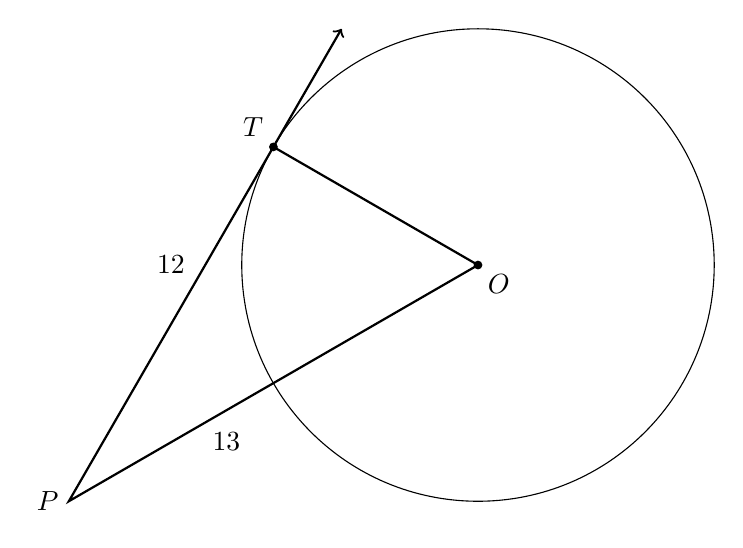
\begin{tikzpicture}[scale=0.6]
        \draw [<-, thick] (120:5.774)--(210:10)node[left]{$P$}
        --(0,0)--(150:5)node[above left]{$T$};
        \draw (0,0) circle [radius=5] node[below right]{$O$};
        %\draw (123:5) ++(-28:0.5)-- ++(-118:0.5)-- +(152:0.5);
        \draw [fill] (0,0) circle [radius=0.08];
        \draw [fill] (150:5) circle [radius=0.08];
        \node at (215:6.5){13};
        \node at (180:6.5){12};
      \end{tikzpicture}
   \end{center}\vspace{3cm}

  \item A pyramid has a 6 foot by 6 foot square base and height 4 feet, as shown. Find the slant length of the pyramid from the center of the side of the base at point $M$ to the vertex $V$.\\[1cm]
    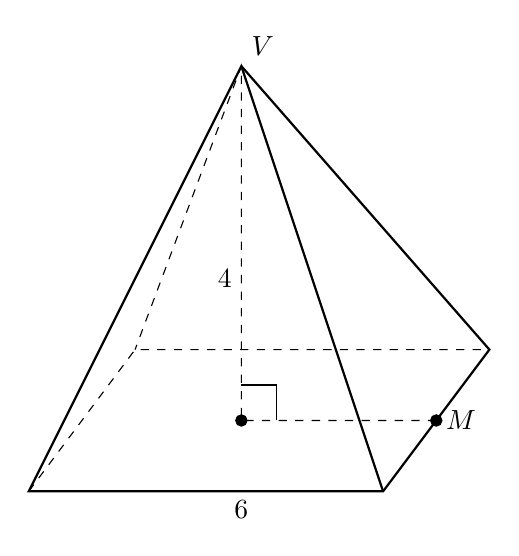
\begin{tikzpicture}[scale=0.9]
      \draw [thick] (-3,-1)--(2,-1)--(3.5,1)--(0,5)node[above right]{$V$}
        --cycle;
      \draw [dashed] (-3,-1)--(-1.5,1)--(3.5,1);
      \draw [thick] (2,-1)--(0,5);
      \draw [dashed] (2.75,0)
        --(0,0)--(0,5)--(-1.5,1);
      \draw (0,0) ++(0:0.5)-- ++(90:0.5)-- +(180:0.5);
      \draw [fill] (0,0) circle [radius=0.08];
      \draw [fill] (2.75,0) circle [radius=0.08]node[right]{$M$};
      \node at (0,2)[left]{4};
      \node at (0,-1)[below]{6};
    \end{tikzpicture}

\newpage
  \item Prove that parallelogram $ABCD$ is a rectangle by showing its diagonals are congruent. Given $A(-5,1)$, $B(-4,4)$, $C(5,1)$, and $D(4,-2)$, as shown below.
    \begin{multicols}{2}
      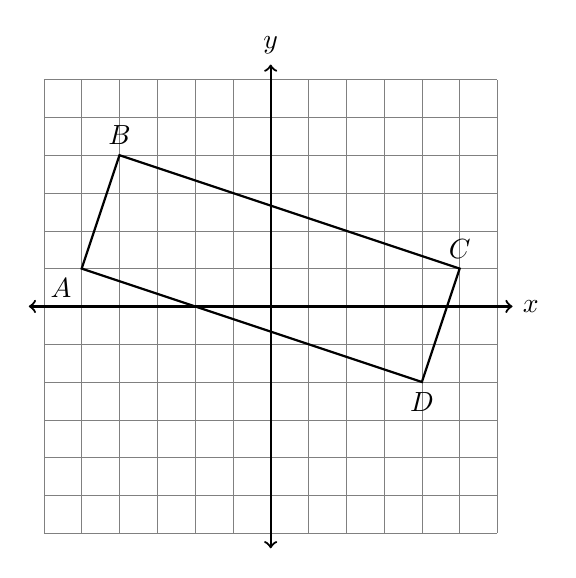
\begin{tikzpicture}[scale=.48]
        \draw [help lines] (-6,-6) grid (6,6);
        \draw [thick, <->] (-6.4,0) -- (6.4,0) node [right] {$x$};
        \draw [thick, <->] (0,-6.4)--(0,6.4) node [above] {$y$};
          \draw [thick]
          (-5,1) node[below left] {$A$}--
          (-4,4) node[above] {$B$}--
          (5,1) node[above] {$C$}--
          (4,-2) node[below] {$D$}--cycle;
      \end{tikzpicture}
      Checklist. Confirm that you...
      \begin{itemize}
        \item Calculate the lengths of the diagonals, $AC$ and $BD$
        \item State that the diagonals are congruent
        \item Write a concluding statement, that therefore parallelogram $ABCD$ is a rectangle because it has congruent diagonals.
      \end{itemize}
    \end{multicols}


\end{enumerate}
\newpage
\setcounter{page}{1}
\subsubsection*{13.8 Exit Note Quiz: Cross sections, distance applications}
Use only a compass and straightedge for these constructions. [show the compass marks]
 \begin{enumerate}

   \item Construct a square, inscribed in circle $O$.
     \vspace{1cm}
     \begin{center}
     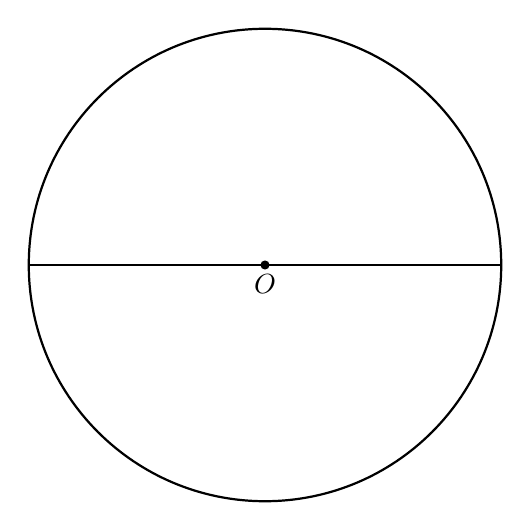
\begin{tikzpicture}
     \draw [thick] (0,0) circle [radius=3cm];
     \draw [thick] (-3,0)--(3,0);
     \draw [fill] (0,0) circle [radius=0.05] node[below]{$O$};
     \end{tikzpicture}
     \end{center}
        \vspace{1cm}

   \item Construct a line through the point $P$ that is parallel to the given line $l$.
     \vspace{3cm}
     \begin{center}
     \begin{tikzpicture}
       \draw [<->, thick] (0,0)--(12,0)node[below]{$l$};
       \draw [fill] (5,3) circle [radius=0.05] node[above left]{$P$};
     \end{tikzpicture}
   \end{center} \vspace{3cm}

\newpage
 \item Find the length of the line segment $\overline{AB}$, with $A(1,3)$ and $B(6,-2)$. Simplify the radical. \vspace{5cm}

 \item Are the given right triangles congruent? $\triangle ABC$ with $m\angle C=90^\circ$, $AC=8$, and $BC=15$. And $\triangle DEF$ with $m\angle E=90^\circ$, $DF=17$, and $EF=15$. \\[0.5cm]
 Justify your answer. \vspace{0.5cm}
   \begin{center}
     \begin{tikzpicture}[scale=0.4]
       \draw [thick] (-8.5,0)node[below]{$A$}
       --(123:8.5)node[above left]{$C$}
       --(8.5,0)node[right]{$B$}--cycle;
       %\draw (0,0) circle [radius=5] node[below]{$O$};
       \draw (123:8.5) ++(-28:0.8)-- ++(-118:0.8)-- +(152:0.8);
       \node at (70:5){15};
       \node at (150:8.5){8};
       \draw [thick] (-12,0)node[below]{$E$}
       --(-20,0)node[left]{$D$}
       --(-12,15)node[right]{$F$}--cycle;
       \draw (-12,0) ++(-180:0.8)-- ++(90:0.8)-- +(0:0.8);
       \node at (-12,7)[right]{15};
       \node at (-16.5,7)[left]{17};
     \end{tikzpicture}
  \end{center}\vspace{5cm}

\newpage
  \item Prove that $\triangle ABC$ is an isosceles triangle but not equilateral, given $A(-5,-2)$, $B(5,0)$, and $C(-1,4)$, as shown below.
    \begin{multicols}{2}
      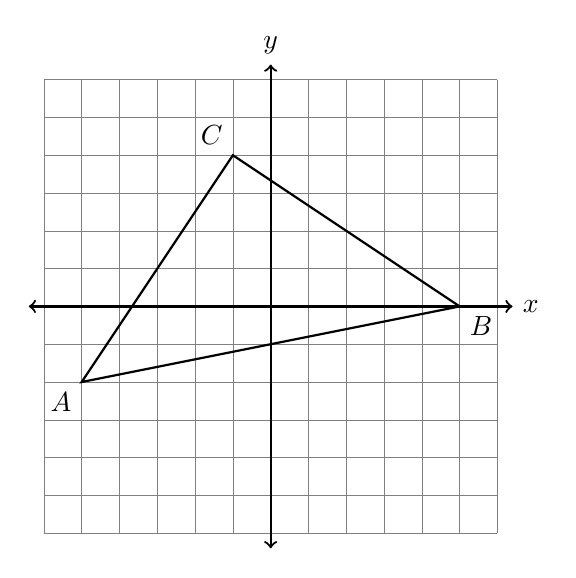
\begin{tikzpicture}[scale=.48]
        \draw [help lines] (-6,-6) grid (6,6);
        \draw [thick, <->] (-6.4,0) -- (6.4,0) node [right] {$x$};
        \draw [thick, <->] (0,-6.4)--(0,6.4) node [above] {$y$};
          \draw [thick]
          (-5,-2) node[below left] {$A$}--
          (5,0) node[below right] {$B$}--
          (-1,4) node[above left] {$C$}--
          cycle;
      \end{tikzpicture}
      Checklist. Confirm that you...
      \begin{itemize}
        \item Calculate lengths $AB$, $AC$ and $BC$\\
        (you do not have to simplify the radical)
        \item State which sides are congruent and which are not
        \item Write a concluding statement, that therefore $\triangle ABC$ is an isosceles triangle but not equilateral.
      \end{itemize}
    \end{multicols}

\newpage
  \item Which three-dimensional figure will result when a rectangle 6 inches long and 5 inches wide is continuously rotated about the longer side?
    \begin{enumerate}
      \item a rectangular prism with a length of 6 inches, width of 6 inches, and height of 5 inches
      \item a rectangular prism with a length of 6 inches, width of 5 inches, and height of 5 inches
      \item a cylinder with a radius of 5 inches and a height of 6 inches
      \item a cylinder with a radius of 6 inches and a height of 5 inches
    \end{enumerate} \vspace{1cm}

 \item An isosceles right triangle whose legs measure 6 is continuously rotated about one of its legs to form a three-dimensional object. The three-dimensional object is a
  \begin{enumerate}
    \item cylinder with a diameter of 6
    \item cylinder with a diameter of 12
    \item cone with a diameter of 6
    \item cone with a diameter of 12
  \end{enumerate} \vspace{1cm}

 \item A right cylinder is cut perpendicular to its base. The shape of the cross section is a
  \begin{enumerate}
    \item circle
    \item cylinder
    \item rectangle
    \item triangular prism
  \end{enumerate} \vspace{1cm}

 \item Simplify each expression. (Leave it in radical form if necessary, not a decimal.)
  \begin{enumerate}
    \begin{multicols}{2}
    \item   $\sqrt{48}$ \vspace{1.25cm}
    \item   $\sqrt{32}$ \vspace{1.25cm}
    \end{multicols}
  \end{enumerate}

\end{enumerate}
\end{document}
